\documentclass[aps,prc,reprint,amsmath,nofootinbib]{revtex4-1}

\usepackage[utf8]{inputenc}
\usepackage{amsmath}
\usepackage{amssymb}
\usepackage{multirow}

\usepackage[inline]{enumitem}

\usepackage{color}
\definecolor{theblue}{RGB}{0,50,230}

\usepackage[pdfencoding=auto, psdextra]{hyperref}

\hypersetup{
  colorlinks=true,
  linkcolor=theblue,
  citecolor=theblue,
  urlcolor=theblue
}

\usepackage{tikz}

\usepackage{graphicx}
\graphicspath{{../plots/}{/fig/}}

\newcommand{\trento}{T\raisebox{-0.5ex}{R}ENTo}
\newcommand{\avg}[1]{\langle #1 \rangle}
\newcommand{\nch}{N_\text{ch}}
\newcommand{\npart}{N_\text{part}}
\newcommand{\sqrts}{\sqrt{s_{NN}}}
\newcommand{\T}{\tilde{T}}
\newcommand{\x}{\mathbf{x}}
\newcommand{\vnk}[2]{v_#1\{#2\}}
\newcommand{\paddedhline}{\noalign{\smallskip}\hline\noalign{\smallskip}}
\newcommand{\order}[1]{$\mathcal O(10^{#1})$}
\newcommand{\note}{\textcolor{theblue}{[?]}}
\newcommand{\smaller}[1]{{\small #1}}

% hyperref throws warning when a line break is used in the title
% this removes the warning by redefining the line break in a pdf string
\pdfstringdefDisableCommands{%
  \def\\#1{ #1}
}

% Convenient figure macro.  Usage:
%
%   \fig[placement specifier = t]{filename}{caption}
%
% This creates a figure environment, includes the given filename as graphics,
% puts the given caption below the graphics, and labels it 'fig:filename'.
% The optional placement specifier defaults to 't' and is passed directly to
% the figure environment.
% Use \fig* to make a figure* environment, i.e. a wide figure.
\usepackage{xparse}
\NewDocumentCommand\fig{sO{t}mm}{
  \begin{figure\IfBooleanT{#1}{*}}[#2]
    \includegraphics{#3}
    \caption{\label{fig:#3}#4}
  \end{figure\IfBooleanT{#1}{*}}
}


\begin{document}

\title{
  Estimating initial state and quark-gluon plasma medium properties\\
  using a hybrid model with nucleon substructure\\
  calibrated to p-Pb and Pb-Pb collisions at \texorpdfstring{$\mathbf{\sqrts=5.02}$}{}~TeV
}

\author{J.\ Scott Moreland}
\author{Jonah E.\ Bernhard}
\author{Steffen A.\ Bass}

\affiliation{Department of Physics, Duke University, Durham, NC 27708-0305}

\date{\today}

\begin{abstract}
  We posit a unified hydrodynamic and microscopic description of the quark-gluon plasma (QGP) produced in ultrarelativistic p-Pb and Pb-Pb collisions at $\sqrts=5.02$~TeV and evaluate our assertion using Bayesian inference. Specifically, we model the dynamics of both collision systems using initial conditions with parametric nucleon substructure, a pre-equilibrium free-streaming stage, event-by-event viscous hydrodynamics, and a microscopic hadronic afterburner.
Free parameters of the model which describe the initial state and QGP medium are then simultaneously calibrated to fit charged particle yields, mean $p_T$ and flow cumulants.
We argue that the global agreement of the calibrated model with the experimental data strongly supports the existence of hydrodynamic flow in small collision systems at ultrarelativistic energies, and that this flow necessarily develops at length scales smaller than a proton.
Posterior estimates for the model's input parameters are obtained, and new insights into the temperature dependence of the QGP transport coefficients and event-by-event structure of the proton are discussed.
\end{abstract}

\maketitle

\section{Introduction}

Ultrarelativistic nuclear collisions between one light-ion and one heavy-ion, e.g.\ $^3$He-Au and p-Pb collisions, generate dense, compact sources of nuclear matter which produce long-range multiparticle correlations that are strikingly similar to the correlations observed in heavy-ion collisions where collectivity is commonly explained by the existence of hydrodynamic flow \cite{CMS:2012qk, Abelev:2012ola, Aad:2012gla, Adare:2015ctn}.
This observation suggests that hydrodynamic behavior could be manifest in small droplets of quark-gluon-plasma (QGP), and that flow might develop at length scales smaller than a single proton.

Hydrodynamic models of ultrarelativistic nuclear collisions are complicated by a number of theoretical unknowns, including the detailed geometry of the QGP initial conditions, the strength and duration of pre-equilibrium dynamics, the temperature dependence of QGP transport coefficients, and the boundaries of hydrodynamic applicability \cite{Niemi:2014lha, deSouza:2015ena, Ollitrault:2012cm, Song:2012ua}.
In general, these theoretical uncertainties tend to grow with decreasing system size, where emergent physics at sub-fermi length scales becomes important to describe bulk properties of the produced system.

One method for reducing theoretical uncertainties is to test model calculations by varying the species of colliding nuclei at a single beam energy \cite{Adare:2015bua, Schenke:2014tga, Aidala:2018mcw, Adare:2017wlc, Adamczyk:2015obl, Shen:2016zpp, Aidala:2017ajz, Adare:2006ti}.
Since initial condition and hydrodynamic models generally factorize the structure of the colliding nuclei from the subsequent time dynamics of the collision, a single theory framework can be simultaneously tested and compared to measurements from multiple collision systems using a self-consistent set of model parameters where only the nuclear structure in the model is permitted to vary.

Typically, the macroscopic structure of heavy nuclei, characterized e.g.\ by an atomic mass and set of Woods-Saxon coefficients \cite{MOLLER1995185, DEVRIES1987495}, is regarded as a known input to hydrodynamic models which contributes negligible uncertainty to simulation predictions, outweighed by large uncertainties in modeling initial energy deposition and off-equilibrium dynamics \cite{Niemi:2014lha, Song:2011hk, Retinskaya:2013gca, Liu:2015nwa, Kurkela:2016vts}.
The geometry of light ions, meanwhile, is naturally more sensitive to the detailed size and shape of individual protons and neutrons inside the nucleus, which may fluctuate event-by-event and differ signficantly from the round blobs typically used to approximate nucleons in heavy-ion collisions \cite{Schenke:2014zha, Welsh:2016siu, Moreland:2017kdx, Schenke:2014gaa, Schlichting:2014ipa}.
These nucleon substructure properties are difficult to measure and calculate from first principles and hence contribute significant uncertainty to model predictions of small systems.

Early substructure studies replaced round protons with composite protons, described by a few salient model parameters, in order to investigate the effect of each parameter on simulated observables \cite{Adler:2013aqf, Mitchell:2016jio, Welsh:2016siu}.
These sensitivity studies were able to identify cause and effect relationships between model inputs and outputs, but lacked the ability to constrain nucleon substructure parameters in any kind of global or systematic fashion.
It quickly became apparent that numerous substructure implementations might be compatible with available data, and that additional work would be required to identify observables which are particularly sensitive to the average size, shape and fluctuations of the proton.

Several such observables have been identified in proton-proton and proton-lepton scattering data.
Measurements by the TOTEM collaboration at $\sqrt{s}=7$~TeV, for instance, found an unexpected dip in the inelasticity density of $p$-$p$ collisions at zero impact parameter \cite{Antchev:2011zz}.
It was later realized that this depression, or so-called hollowness effect in the $p$-$p$ inelastic collision profile \cite{Arriola2016}, can be explained by the existence of correlated domains inside the proton, and that aspects of these domains, such as their size and correlation strength, may be constrained by comparing model predictions to inelastic $p$-$p$ measurements \cite{Albacete:2016gxu, Albacete:2016pmp}.

Independently, studies of coherent and incoherent $J/\psi$ production based on a color dipole picture of vector meson production were used to simultaneously constrain both the average color charge density of the proton as well as its event-by-event fluctuations in a saturation based framework \cite{Mantysaari:2016ykx, Aaron:2009aa, Abramowicz:2015mha}.
Initial condition studies using the IP-Glasma model of color-glass condensate effective field theory simultaneously demonstrated that these color charge fluctuations leave a lasting imprint on the \mbox{small-x} gluon distribution of the proton and hence the initial geometry of QGP energy deposition \cite{Schlichting:2014ipa}.
Just recently, hydrodynamic simulations using IP-Glasma initial conditions with color charge fluctuations calibrated to fit coherent and incoherent $J/\psi$ diffraction measured by the H1 and Zeus experiments at HERA \cite{Aaron:2009aa, Abramowicz:2015mha} were shown to provide a good description of collectivity in small and large collision systems \note.

Model parameters are of course always in some degree of tension; for instance, fitting one observable may require parameter values that degrade the quantitative description of some other observable.
Similarly, parameters which provide an optimal description of small-system observables may lead to a sub-optimal description of heavy-ion observables or \emph{vice versa}.
It is thus import to look at the experimental data holistically, and to use model calibration methods which
\begin{enumerate*}[label=(\arabic*)]
  \item explore all parameter combinations and
  \item compare model predictions to all relevant experimental measurements in a statistically rigorous fashion.
\end{enumerate*}

We apply, in this work, a model calibration framework known as Bayesian parameter estimation which is ideally suited for this purpose.
The framework was previously adapted and applied to relativistic heavy-ion collisions, and has since been used in a number of studies to constrain the properties of hot and dense nuclear matter.
We use it in the present study to search for a unified description of $p$-Pb and Pb-Pb collisions at $\sqrts=5.02$~TeV.

%Section 1 describes our nuclear collision model.
%Sections 2 and 3 describe the computer experiment design and model calibration process which is used to obtain posterior estimates of the model input parameters.
%In section 4 we presents the results of our analysis.

%We perform a global analysis of soft-sector observables measured in $p$-Pb and Pb-Pb collisions at $\sqrts=5.02$~TeV and calibrate free parameters of a hybrid transport model to describe the experimental data.
%
%to obtain posterior probability estimates for the model parameters given our chosen model, the experimental data and known sources of uncertainty.


\section{Nuclear collision model}

We employ a multi-stage hybrid transport model that uses relativistic viscous hydrodynamics to describe the QGP medium and microscopic Boltzmann transport to simulate the dynamics of the system after hadronization \note.
The hydrodynamic initial conditions are provided by a modified version of the \trento\ model \cite{Moreland:2014oya} with additional parameters to vary the size and shape of the nucleon.
Each initial condition profile is free streamed to the hydrodynamic starting time and matched onto the hydrodynamic energy-momentum tensor using the Landau matching procedure \note.
All components of the present model, with the exception of the nucleon substructure implementation, are documented in previous studies \note. We review them here for clarity.

\subsection{Initial state}

We model the QGP initial state in $p$-Pb and Pb-Pb collisions at $\sqrts=5.02$~TeV using a simple parametric form for boost-invariant entropy deposition employed by the \trento\ model \cite{Moreland:2014oya}.
Generally speaking, the initial three-dimensional distribution of matter produced in relativistic nuclear collisions is \emph{not} boost-invariant; longitudinal entropy deposition fluctuates both locally point-to-point in the transverse plane as well as globally event-by-event due to asymmetries in the sampled density of participant matter \note.
Nevertheless, boost-invariance has been shown to be a good approximation for both large and small collision systems when hydrodynamic observables are calculated from particles that are detected close to midrapidity \note.

The \trento\ model operates in the ultrarelativistic limit with a Lorentz factor $\gamma \gg 1$ such that each nucleus appears as a thin sheet of nuclear density in the laboratory frame.
The sheets of colliding nuclear density penetrate and pass through each other in time $\Delta t = D_\text{nucl} / \sqrt{\gamma^2 - 1}$ in the laboratory frame, where $D_\text{nucl}$ is the diameter of the nucleus in its rest frame and $\gamma$ is the usual Lorentz factor of the accelerated ions.
The resulting nuclear overlap time $\Delta t \lesssim 0.1$~fm/$c$ at top RHIC and LHC energies is thus sufficiently short to neglect initial transverse dynamics which occur while the nuclei pass through each other.
We therefore assume that the collision produces all secondary particles at uniform proper time $\tau = 0^+$~fm/$c$, and that it deposits entropy (energy) at midrapidity which is a function of the locally varying beam integrated density of each nucleus.

Consider the collision of two protons $A$, $B$ with three-dimensional densities $\rho_{A,B}$ in their local rest frames.
The proton-proton overlap function
\begin{equation}
  \label{Tpp}
  T_{pp}(b) \equiv \int dx\, dy \int dz\, \rho_A(\x) \int dz\, \rho_B(\x + \mathbf{b}),
\end{equation}
describes the eikonal overlap of the two proton wave packets at fixed impact parameter $b$ where coordinates $(x, y)$ lie in the transverse plane and $z$ is parallel to the beam axis.
Here we assume that each proton is comprised of smaller constituents---e.g.\ valence quarks, sea quarks, and small-x gluons---which may collide to produce secondary particles and contribute to the observed inelastic proton-proton cross section.

Within a picture of independent pairwise collisions between the constituents, a Glauber model model may be used to calculate the probability $P_\mathrm{coll}$ that the two protons collide inelastically at impact parameter $b$. In the limit when the number of constituents $M \gg 1$, it yields the particularly simple form
\begin{equation}
  \label{Pcoll}
  P_\mathrm{coll} = 1 - \exp[-\sigma_\mathrm{eff}\, T_{pp}(b)], \\
\end{equation}
where $\sigma_\mathrm{eff}$ is an effective cross section for pairwise inelastic collisions between the constituents, and $\sigma_{pp}^\mathrm{inel}$ is the total inelastic proton-proton cross section:
\begin{equation}
  \label{sigma_nn}
  \sigma_{pp}^\mathrm{inel} = \int 2 \pi b\, db\, P_\mathrm{coll}(b).
\end{equation}
The proton densities $\rho_{A,B}$ in Eqn.~\eqref{Tpp} are commonly modeled using a spherically symmetric distribution \note.
For instance, the original implementation of the \trento\ model uses Gaussian protons, largely because it yields a simple analytic solution to Eqn.~\eqref{Pcoll}.
Needless to say, such approximations are admittedly crude and may have a significant effect on the dynamics of small collision systems where the proton size is comparable to the size of the produced QGP medium.

Several previous studies have investigated the effects of deformed or ``lumpy'' protons \note.
One common implementation is a superposition of three valence quarks, typically described by Gaussian or exponential form factors.
The corresponding proton density $\rho(\mathbf{x})$ is then assumed to be that of predominantly small-x gluons, seeded by the distribution of color charge in each of the three valence quarks \note.

\begin{figure}
  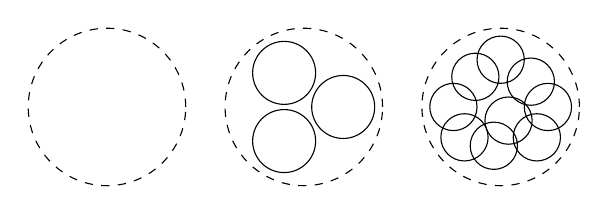
\begin{tikzpicture}
    % spherical proton
    \draw[dashed, xshift=-2.5cm] (0,0) circle (1cm);
    % three partons
    \draw[dashed] (0,0) circle (1cm);
    \foreach \theta in {0, 120, 240}{
      \draw ({\theta}:.5) circle (.4cm);
    }
    % ten partons
    \draw[dashed, xshift=2.5cm] (0,0) circle (1cm);
    \foreach \theta/\radius in {
      0/0.6, 40/0.5, 90/0.6, 130/0.5, 180/0.6, 220/0.6,
      260/0.5, 320/0.6, 300/0.2
    }{
      \draw[xshift=2.5cm] ({\theta}:\radius) circle (.3cm);
    }
  \end{tikzpicture}
  \caption{\label{fig:substructure} Schematic of plausible proton shapes.
  The sketch on the left shows a spherically symmetric proton (dashed line), while the middle and right illustrations depict a fluctuating proton with three and nine constituents respectively (solid lines).
  }
\end{figure}

In this work, we pursue a less restrictive and more parametric description of the proton where the number of substructure degrees of freedom are uncertain as depicted in Fig.~\ref{fig:substructure}.
We model each nucleon's density $\rho_{A,B}$ as a sum of $M$ independent constituents
\begin{equation}
  \label{rho}
  \rho_{A, B}(\x) = \frac{1}{M} \sum\limits_{i=1}^M \rho_c(\mathbf{x} - \mathbf{x_i}),
\end{equation}
where each constituent density $\rho_c$ is described by a Gaussian distribution of width $w$
\begin{equation}
  \rho_c(\mathbf{x}) = \frac{1}{(2\pi w^2)^{3/2}} \exp\left(-\frac{\x^2}{2 w^2}\right),
\end{equation}
and each constituent's position $\mathbf{x_i}$ in Eqn.~\eqref{rho} is sampled from a Gaussian radial distribution of width $r$.
In the limit $M\to \infty$, the composite proton's root mean square radius is simply the convolution of its sampling radius and constituent width, which add together in quadrature
\begin{equation}
  \lim_{M\to\infty} \mathrm{RMS}\{\rho(\mathbf{x})\} = \sqrt{r^2 + w^2}.
\end{equation}
We therefore choose to reparametrize the sampling radius $r$ in terms of the variable $\sigma = \sqrt{r^2 - w^2}$ which approximates the proton's root mean square radius when the number of sampled constituents is large.

The two protons $A$, $B$ are assigned a random impact parameter, and Eqn.~\eqref{Pcoll} is used to sample their inelastic collision probability $P_\mathrm{coll}(b)$.
Note that this proton-proton inelastic collision probability has no direct knowledge of the individual constituent degrees of freedom; it is only \emph{indirectly} sensitive through the geometry of $\rho_{A, B}$ which depends on each of the constituent positions.
This is an important distinction between the present model and a similar nucleon substructure implementation known as the participant or ``wounded'' quark model which allows for a subset of quarks (constituents) to participate inside a single nucleon \note.
The proton, unlike the nucleus, cannot produce semi-stable spectator fragments in a high-energy collision.
Any spectator quarks produced by a wounded quark model would be colored objects that necessarily contribute to secondary particle production as they fragment and recombine to form color-neutral hadrons.
We correspondingly require that the nucleons in Eqn.~\eqref{rho} participate as singular objects, such that all spectator matter discarded by the simulation is appropriately color-neutral and inert.

Assuming our two protons collide at the sampled impact parameter $\mathbf{b}$, we assign each a \emph{fluctuated} thickness
\begin{equation}
  \label{fluctuated_thick}
  \T_{A, B}(\x) \equiv \int dz\, \frac{1}{M} \sum\limits_{i=1}^M \gamma_i\, \rho_c \,(\mathbf{x} - \mathbf{x_i} \pm \mathbf{b}/2),
\end{equation}
equal to the beam-integrated proton density in Eqn.~\eqref{rho}, with each constituent shifted by the appropriate impact parameter offset, and multiplied by a gamma random variable $\gamma_i$ with unit mean and variance $1/k$.
These \emph{ad hoc} gamma random weights are necessary to describe the large fluctuations observed in minimum bias proton-proton collisions, although their physical justification is not yet well understood.

Within the eikonal approximation, the initial entropy deposited at midrapidity at proper time $\tau=0^+$~fm/$c$ can be represented by some mapping ${f(\T_A, \T_B) \mapsto dS/dy}$.
A natural first guess for the function $f$ is an arithmetic mean $f \propto (\T_A + \T_B)/2$, equal to a wounded nucleon model up to meaningless factor of two in the overall normalization.
The wounded nucleon model was in fact the first such mapping used as a proxy for initial particle production and entropy deposition in relativistic heavy-ion collisions \note.
It was quickly realized, however, that the wounded nucleon model predicts the wrong scaling for charged particle production as a function of collision centrality and hence the wrong scaling for initial entropy deposition as a function of participant thickness $\T_{A,B}$ \note.

A simple remedy is to replace the arithmetic mean in the wounded nucleon model with a more flexible parametrization
\begin{equation}
  \label{gmean}
  \frac{dS}{dy}\bigg\vert_{y=0} \propto \left( \frac{\T_A^p + \T_B^p}{2} \right)^{1/p},
\end{equation}
based on a family of functions known as the generalized mean(s).
This parametrization introduces a dimensionless parameter $p$ which varies the scaling behavior of initial entropy deposition at midrapidity.
For certain discrete values of $p$, it reduces to well known functional forms such as the arithmetic, geometric and harmonic means:
\begin{equation}
  \newlength{\extraspace}
  \setlength{\extraspace}{0.5ex}
  \frac{dS}{dy}\bigg\vert_{y=0} \propto
  \begin{cases}
    \max(T_A, T_B) & p \rightarrow +\infty, \\[\extraspace]
    (T_A + T_B)/2 & p = +1, \hfill \text{ (arithmetic)} \\[\extraspace]
    \sqrt{T_A T_B} & p = 0, \hfill \text{ (geometric)} \\[\extraspace]
    2\, T_A T_B/(T_A + T_B) & p = -1, \hfill \text{ (harmonic)} \\[\extraspace]
    \min(T_A, T_B) & p \rightarrow -\infty.
  \end{cases}
\end{equation}
Conveniently, it has been shown that the generalized mean ansatz is able to mimic the scaling behavior of certain saturation based initial condition models \note, and hence it should serve as a reasonable parametric form for exploring QGP entropy deposition, assuming imperfect knowledge of saturation effects in nature.
Of course the model is \emph{not} a substitute for first principle saturation calculations, and may fail to reproduce nuanced features of \emph{ab initio} saturation theory calculations, such as the existence of short-range gluon field fluctuations \note.

\begin{figure}
  \centering
  \begin{tikzpicture}
    \node {\includegraphics[width=\columnwidth]{fig/thickness}};
    \node[label=above:{10 fm}] (a) at (0, 1.1) {};
    \node (b) at (0, -1.1) {};
    \draw [<->, semithick] (a) to (b);
  \end{tikzpicture}
  \caption{\label{fig:substructure} Effect of nucleon substructure on the nuclear thickness function $T(x, y) \equiv \int dz\, \rho(x, y, z)$ of a $^{208}\mathrm{Pb}$ nucleus.
    The nucleus on the left has Gaussian nucleons of width $0.88$~fm, while the nucleus on the right has composite nucleons, each containing six Gaussian constituents of width $0.41$~fm.}
\end{figure}

Equation~\eqref{gmean} is a purely local function of nuclear density in the transverse plane and should (in principle) be equally valid for any pair of colliding nuclei at sufficiently high beam energy.
The model readily generalizes from individual proton-proton collisions to arbitrary nucleus-nucleus collisions by summing the participant thicknesses $\T_{A,B}$ over all nucleons which participate in one or more inelastic collisions.
The only modeling difference between $p$-$p$ collisions and Pb-Pb collisions is the number and the position of the nucleons.

When applying the model to heavy-ions, we sample nucleon positions from a Woods-Saxon density distribution subject to a minimum distance criteria $|\mathbf{x_i} - \mathbf{x_j}| > d_\mathrm{min}$ between all pairs of nucleons $i$, $j$.
The minimum distance algorithm, first described in Ref.~\note, uses a simple trick to resample the nucleon positions without modifying the target Woods-Saxon radial distribution.
We first presample the radii of all nucleons in a given nucleus and sort them in ascending order.
We then sample the solid angles of each nucleon one-by-one, starting with the nucleon closest to the center of the nucleus and working our way outwards.
If a sampled nucleon position is too close to any of its previously placed neighbors, its solid angle is resampled until the minimum distance criteria is satisfied.
Similar methods could be used to model correlations between individual constituents inside each nucleon, although the numerical implementation would be somewhat tedious.

\subsection{Pre-equilibrium dynamics}

\begin{figure}[b]
  \includegraphics{fig/coupling}
  \caption{\label{fig:freestream} Cartoon of the free-streaming approximation for hydrodynamic initialization. The initial state is free-streamed for proper time $\tau_{fs}$ (zero-coupling) before it is matched to hydrodynamics (strong-coupling). This piecewise evolution approximates the more realistic scenario expected in nature where the medium's coupling strength smoothly changes as a function of time.}
\end{figure}

There are of course two limiting cases for the strength of interactions inside the QGP medium immediately at the collision: infinitely weak coupling where the secondary partons free-stream without interacting, and infinitely strong coupling where the fluid's inter-particle mean free path effectively vanishes.
Realistically, one expects the initial parton interactions to lie somewhere between these two extremes.
We therefore choose to model the QGP's initial off-equilibrium dynamics using a simple step-function approximation, depicted in Fig.~\ref{fig:freestream}, which free-streams the initial state for proper time $\tau_{fs}$ (zero coupling) before instantaneously switching to viscous hydrodynamics (strong coupling) \note.
The free parameter $\tau_{fs}$ allows us to parametrically vary the \emph{time averaged} coupling strength in the approximate window $0 < \tau_{fs} \lesssim1$~fm/$c$.

The parametric entropy deposition ansatz in Eqn.~\eqref{gmean} does not provide any information about the initial masses or momenta of particles produced in the collision.
In general, these details will affect the dynamics predicted by the collisionless Boltzmann equation
\begin{equation}
  \label{freestream}
  p^\mu \partial_\mu f(x, p) = 0,
\end{equation}
through its dependence on the underlying distribution function $f(x, p)$, and hence are necessary inputs for any free-streaming implementation.
Equation~\eqref{freestream}, however, simplifies for massless partons with momentum distributions that are locally isotropic.
Under this assumption, it was shown in Refs.~\cite{Broniowski:2008qk, Liu:2015nwa} that the energy-momentum tensor $T^{\mu\nu}$ of partons at midrapidity and time $\tau$ only depends on its spatial distribution at some earlier time $\tau_0$, but not its $p_\perp$-distribution, which could vary as a function of position.

We thus follow the procedure of the authors and reinterpret our initial transverse entropy density at midrapidity $s(\mathbf{x_\perp}, \tau_0)\vert_{\eta=0}$ as a transverse density of noninteracting massless partons $n(\mathbf{x}, \tau_0)\vert_{\eta=0}$.
The free-streamed energy-momentum tensor $T^{\mu\nu}(x, y, \eta, \tau)$ at transverse coordinate $(x, y)$, midrapidity $\eta=0$, and proper time $\tau > \tau_0$ is then given by
\begin{multline}
  \label{energy-momentum}
  T^{\mu\nu}(x, y, 0, \tau) = \frac{1}{\tau} \int_{0}^{2\pi} d\phi\, n(x - \Delta \tau \cos \phi, y - \Delta \tau \sin \phi) \\ \times
  \begin{bmatrix}
    1 & \cos\phi & \sin\phi  & 0\\
    \cos\phi & \cos^2\phi & \cos\phi\sin\phi & 0 \\
    \sin\phi & \sin\phi \cos\phi & \sin^2\phi & 0\\
    0 & 0 & 0 & 0
  \end{bmatrix},
\end{multline}
where $\Delta\tau$ is the free-streaming time $\Delta\tau = \tau - \tau_0$.
The solution \eqref{energy-momentum} is decomposed in hydrodynamic form
\begin{equation}
  \label{hydro-eqn}
  T^{\mu\nu} = e u^\mu u^\nu - (P + \Pi) \Delta^{\mu\nu} + \pi^{\mu\nu}
\end{equation}
where $e$ and $P$ are the energy density and pressure in the local fluid rest frame, $u^\mu$ is the local fluid velocity, ${\Delta^{\mu\nu} \equiv g^{\mu\nu} - u^\mu u^\nu}$, and $\Pi$ and $\pi^{\mu\nu}$ are the bulk pressure and shear stress tensor respectively.
We then solve for the energy density $e$ and fluid velocity $u^\mu$ using the Landau matching condition which defines the fluid rest frame velocity as the time-like eigenvector of $T^{\mu\nu}$ with energy density $e$ as its eigenvalue,
\begin{equation}
  T^{\mu\nu} u_\nu = e u^\mu.
\end{equation}
The initial bulk and shear corrections are finally solved for by subtracting the ideal pressure from the total pressure to find $\Pi$, then solving for $\pi^{\mu\nu}$ using Eqn.~\eqref{hydro-eqn}
\begin{align}
  \Pi &= -\frac{1}{3} \mathrm{Tr}(\Delta_{\mu\nu} T^{\mu\nu}) - P,\\
  \pi^{\mu\nu} &= T^{\mu\nu} - e u^\mu u^\nu + (P + \Pi) \Delta^{\mu\nu}.
\end{align}

This procedure provides initial values for $T^{\mu\nu}$, $u^\mu$, $\Pi$ and $\pi^{\mu\nu}$ which conserve energy and are consistent with the underlying hydrodynamic equation of state.
We therefore expect it to provide a more realistic description of the initial stages of the collision as compared to a previous study using the \trento\ initial condition model which set $\Pi$, $\pi^{\mu\nu}$ and $u^\mu$ initially to zero \cite{Bernhard:2016tnd}.


\subsection{Hydrodynamics}

After free-streaming for proper time $\tau_{fs}$, we transition to viscous hydrodynamics which solves the conservation equations
\begin{equation}
  \label{eq:continuity}
  \partial_\mu T^{\mu\nu} = 0
\end{equation}
for the hydrodynamic energy-momentum tensor $T^{\mu\nu}$ expressed in Eqn.~\eqref{hydro-eqn} using a set of second-order Israel-Stewart equations formulated in the 14-moment approximation
\cite{Israel:1979wp, Israel:1976aa, Denicol:2012cn, Denicol:2010xn}.
This produces a pair of relaxation-type equations
\begin{subequations}
  \label{eq:relaxation}
  \begin{align}
    \tau_\Pi \Pi + \dot{\Pi} &=
      - \zeta \theta - \delta_{\Pi\Pi} \Pi\theta
      + \lambda_{\Pi\pi} \pi^{\mu\nu} \sigma_{\mu\nu}, \\[1ex]
    \tau_\pi \dot{\pi}^{\langle \mu\nu \rangle} + \pi^{\mu\nu} &=
      2\eta\sigma^{\mu\nu} - \delta_{\pi\pi} \pi^{\mu\nu} \theta
      + \phi_7 \pi_\alpha^{\langle \mu} \pi^{\nu \rangle \alpha} \nonumber \\
      &\qquad {} - \tau_{\pi\pi} \pi_\alpha^{\langle \mu}\sigma^{\nu \rangle \alpha}
      + \lambda_{\pi\Pi} \Pi \sigma^{\mu\nu},
  \end{align}
\end{subequations}
for the bulk pressure $\Pi$ and shear-stress $\pi^{\mu\nu}$.
We model the shear viscosity $\eta$ and bulk viscosity $\zeta$ as unknown temperature dependent quantities and fix the remaining transport coefficients $\{\tau_\Pi, \delta_{\Pi\Pi}, \lambda_{\Pi\pi}, \tau_\pi, \delta_{\pi\pi}, \phi_7, \tau_{\pi\pi}, \lambda_{\pi\Pi}\}$ using analytic results derived in the limit of small but finite masses \cite{Denicol:2014vaa}.

\begin{figure}
  \centering
  \includegraphics{fig/viscosity_dof}
  \caption{\label{fig:viscosity_dof} Degrees of freedom in the temperature dependent shear and bulk viscosity parametrizations.
  Lines are chosen for illustrative purposes only and do not represent all possible variability.
  For instance, $\eta/s$ could have a large slope and negative curvature, or $\zeta/s$ could have a large max and narrow width, neither of which are depicted above.
}
\end{figure}

The hydrodynamic equations of motion are necessarily closed using an equation of state (EoS) to relate the energy density $e$ and pressure $P$ of the produced medium.
We use a parametrization for $P(e)$ that matches a hadron resonance gas EoS at low temperature to a lattice QCD EoS at high temperature by smoothly connecting their trace anomalies in the interval $165 \le T \le 200$~MeV.
For the lattice EoS, we use a calculation by the HotQCD collaboration for (2+1)-flavor QCD which was extrapolated to the continuum limit \cite{Bazavov:2014pvz}. Recent developments in lattice QCD now enable calculations in (2+1+1)-flavors \cite{Borsanyi:2016ksw}, i.e.\ with thermalized charm quarks, and the additional charm flavor has been shown to visibly affect predictions of $p_T$-differential flow observables \cite{Noronha-Hostler:2018zxc}.
Investigating this sensitivity would thus be a natural target for future improvements to the present work.

We parametrize the temperature dependence of the QGP viscosities in order to marginalize over their uncertainty when calibrating to data.
For the specific shear viscosity $\eta/s$, we use a modified linear ansatz
\begin{equation}
  \label{eq:shear_viscosity}
  (\eta/s)(T) = (\eta/s)_\mathrm{min} + (\eta/s)_\mathrm{slope}\cdot(T - T_c)\cdot(T/T_c)^{(\eta/s)_\mathrm{crv}}
\end{equation}
where $\eta/s$ min, slope and curvature are tunable parameters and $T_c=0.154$~GeV is the pseudocritical transition temperature of the HotQCD EoS.
While for the specific bulk viscosity $\zeta/s$, we use an unnormalized Cauchy distribution
\begin{equation}
  \label{eq:bulk_viscosity}
  (\zeta/s)(T) = \frac{(\zeta/s)_\mathrm{max}}{1 + \left(\dfrac{T - (\zeta/s)_{T_0}}{(\zeta/s)_\mathrm{width}}\right)^2},
\end{equation}
described by tunable maximum, width, and location ($T_0$) parameters.
Figure~\ref{fig:viscosity_dof} shows several of the possible curves parametrized by Eqns.~\eqref{eq:shear_viscosity} and \eqref{eq:bulk_viscosity}, although many more are possible.

The aforementioned hydrodynamic equations are solved numerically using the boost-invariant \texttt{VISH2+1} viscous hydrodynamics code \note\ which is documented extensively in Ref.~\note.
We simulate each hydrodynamic event on a spacetime grid with transverse extent $x_\mathrm{max}$, spatial grid step $dx$, and time step $d\tau$ which are optimized \emph{event-by-event} to balance trade-offs between numerical accuracy and computation time (see appendix).
Although these details are somewhat mundane, they are critically important to the present study, since the computation time explodes with the number of grid cells,
\begin{equation}
  \mathrm{cpu~time} \sim n_x^2 n_\tau,
\end{equation}
and $nx$ and $n\tau$ typically have to be quite large to resolve the small length scales associated with nucleon substructure.

\subsection{Particlization and Boltzmann transport}

We evolve the system hydrodynamically down to a pre-specified switching isotherm $T_{sw}$ at which point the medium is converted into particles using the Cooper-Frye formula \note
\begin{equation}
  \label{cooper-frye}
  E \frac{dN_i}{d^3p} = \frac{g_i}{(2\pi)^3} \int_\Sigma f_i(x, p)\, p^\mu\, d^3\sigma_\mu,
\end{equation}
where $i$ is an index over species, $f_i$ is the distribution function of that species, and $d^3\sigma_\mu$ is a volume element of the isothermal hypersurface $\Sigma$ defined by $T_\mathrm{sw}$.
Thermal particles are then sampled in the rest frame of each fluid cell according to a Bose-Einstein or Fermi-Dirac distribution at zero baryon chemical potential
\begin{equation}
  \label{distribution}
  f(m, p) = \frac{1}{\exp(\sqrt{m^2 + p^2}/T) \mp 1},
\end{equation}
where $m$ is the mass of the sampled particle, $p$ is its momentum, and $T$ is the temperature of the fluid cell.

\subsubsection{Sampling with finite resonance widths}

Traditionally, particlization models have sampled resonances using each particle's pole mass in Eqn.~\eqref{distribution}.
This approximation, however, is somewhat crude and has been known to underpredict pion production, particularly at low $p_T$ \note.
We thus follow Ref.~\note, and sample particles with a \emph{distribution} of masses
\begin{equation}
  f(p) = \int dm\, \mathcal{P}(m)\, f(m, p),
\end{equation}
where $\mathcal{P}(m)$ is modeled by a Breit-Wigner distribution
\begin{equation}
  \mathcal{P}(m) \propto \frac{\Gamma(m)}{(m - m_0)^2 + \Gamma(m)^2/4}.
\end{equation}
Here $m_0$ is the resonance's Breit-Wigner mass and $\Gamma(m)$ is its mass-dependent width, for which we use a simple form:
\begin{equation}
  \Gamma(m) = \Gamma_0 \sqrt{\frac{m - m_\mathrm{min}}{m_0 - m_\mathrm{min}}},
\end{equation}
where $\Gamma_0$ is the usual Breit-Wigner width and $m_\mathrm{min}$ is a production threshold equal to the total mass of the lightest decay products.

We tabulate the values of $\{\Gamma_0, m_0, m_\mathrm{min}\}$ for all particles and sample the masses of each particle during particlization \note.
The resonances are then passed to a hadronic transport model, described shortly, which simulates subsequent scatterings and decays.

\subsubsection{Viscous corrections to the distribution function}

When the viscous terms $\pi^{\mu\nu}$ and $\Pi$ are nonzero in Eqn.~\eqref{hydro-eqn}, the distribution function $f$ must be modified to preserve the continuity of $T^{\mu\nu}$ as the system transitions from hydrodynamics to Boltzmann transport.
We perform the appropriate modification using a general method which transforms the momentum vector \emph{inside} the distribution function
\begin{align}
  p_i \rightarrow p'_i &= p_i + \sum\limits_j \lambda_{ij}\, p_j,\\
  \lambda_{ij} &= (\lambda_\mathrm{shear})_{ij} + \lambda_\mathrm{bulk}\, \delta_{ij},
\end{align}
where $\lambda_{ij}$ is a linear transformation matrix consisting of a traceless shear part and a bulk part which is proportional to the identity matrix \note.

We use for the shear viscous correction the form \note
\begin{equation}
  (\lambda_\mathrm{shear})_{ij} = \frac{\tau}{2 \eta} \pi_{ij},
\end{equation}
with a value for $\eta/\tau$ obtained from the noninteracting hadron resonance gas model
\begin{equation}
  \frac{\eta}{\tau} = \frac{1}{15 T} \sum\limits_{sp} g \int \frac{d^3p}{(2\pi)^3}\frac{p^4}{E^2} f_0 (1 \pm f_0).
\end{equation}

For the bulk viscous correction, we use a novel procedure developed by one of the authors of this work \note.

\subsubsection{Hadronic Boltzmann transport}

\vfill

\section{Parameter estimation}


\subsection{Computer experiment design}


\subsection{Gaussian process emulators}

\subsection{Bayesian calibration}

\section{Results}

\subsection{Initial condition properties}

\subsection{QGP medium properties}

\section{Summary and conclusions}

\begin{acknowledgments}
  The authors thank ...
\end{acknowledgments}

\appendix*

\section{Adaptive grid sizing}
\label{appendix}
This is the appendix

\bibliography{trento-substructure}

\end{document}
